\section*{Third Design}
--Talk about basic design difference/advantages here-- 

\subsection*{Pipeling the Critical Path}
--Show differing code here-- \\*



\subsection*{Third Design Timing Analysis}

% Table generated by Excel2LaTeX from sheet 'Sheet1'
\begin{table}[bh]
\caption{Xilinx Timing Report}
\begin{tabular}{c|c}
\centering
           & Timing in (ns) \\
\hline
Minimum Period &     \\

     Slack &     \\

Requrement &        \\

Data Path Delay &     \\
\end{tabular}  
\label{tab:timing3}
\end{table}

According to Table \ref{tab:timing3}, the maximum clock frequency for the this design has been calculated to be approximately:  MHz


\begin{figure}[htp]
  \begin{center}
    \subfigure[Functional block diagram]{\label{subfig:block3-a}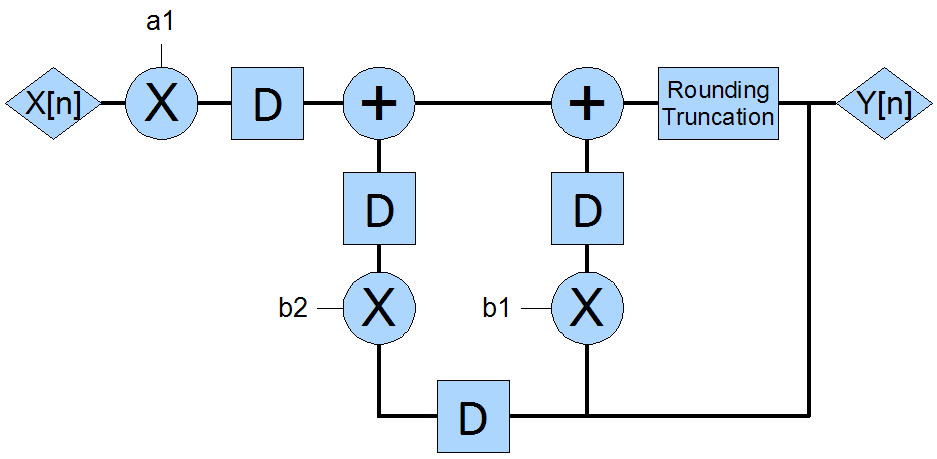
\includegraphics[scale=0.30]{block_three.png}}
    \subfigure[Input/Output comparison]{\label{subfig:output3-b}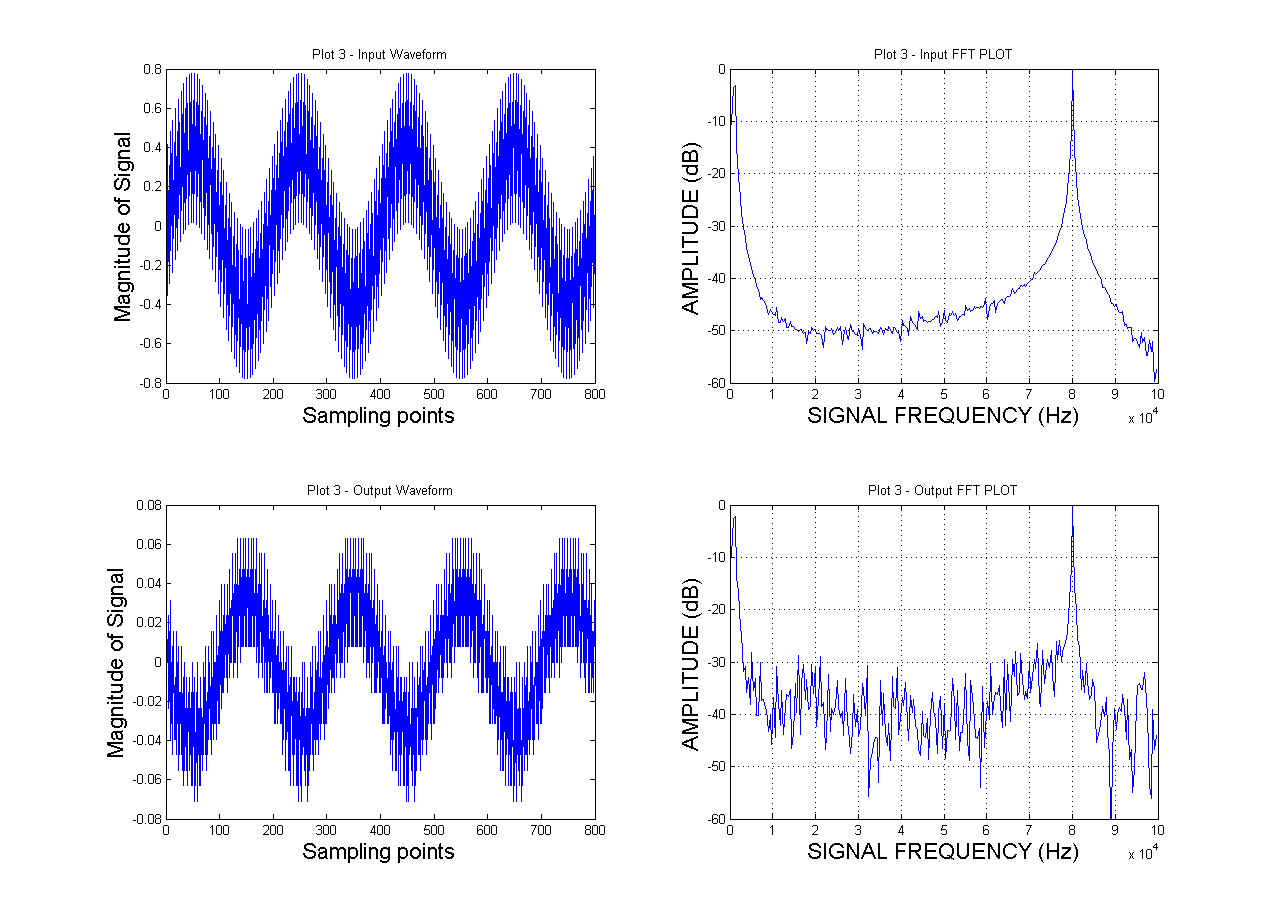
\includegraphics[scale=0.30]{plot3.png}} \\*
  \end{center}
  \caption{Second Design Results}
  \label{fig:design3_results}
\end{figure}